% !TEX TS-program = lualatex

% Основано на  презентациях Юрия Викторовича Литвинова:
% https://github.com/yurii-litvinov/courses/tree/master/programming-1st-semester/12-lists
\documentclass[aspectratio=169]{beamer}

%%% Setup fonts.
\usepackage{fontspec}
%% Fancy fonts
\setmainfont{Iosevka Etoile}
\setsansfont{Iosevka Aile}
\setmonofont{Iosevka}

%% Default fonts
% \setmainfont{CMU Serif}
% \setsansfont{CMU Sans Serif}
% \setmonofont{CMU Typewriter Text}

%% Math
\usepackage{amsmath, amsfonts, amsthm, mathtools} % Advanced math tools.
\usepackage{amssymb}

\usepackage{unicode-math} % Allow TTF and OTF fonts in math and allow direct typing unicode math characters.
\unimathsetup{
    warnings-off={
            mathtools-colon,
            mathtools-overbracket
        }
}
% \setmathfont{Lete Sans Math}[CharacterVariant={3,6},StylisticSet={4}]
\setmathfont{Latin Modern Math}

%%% Language settings.
\usepackage{polyglossia}
\setdefaultlanguage{russian}
\setotherlanguage{english}

%%% Beamer settings
% Themes
\usetheme{Boadilla}
\useinnertheme{circles}
\usecolortheme[style=Latte, accent=Blue]{catppuccin}
% Templates
\setbeamertemplate{navigation symbols}{} %remove navigation symbols
\setbeamertemplate{page number in head/foot}[appendixframenumber]
\setbeamertemplate{title page}[default][colsep=-4bp,rounded=true]

%%% Colors
\hypersetup{colorlinks}
\usepackage{catppuccinpalette}

\usepackage{booktabs}

\usepackage{minted}
\usemintedstyle{catppuccin-latte}

\usepackage{csquotes}

% \usepackage{xurl}

%% Custom commands
\NewDocumentCommand{\attribution}{mmmmm}{\href{#1}{#2}, \href{#3}{#4}, #5}
\NewDocumentCommand{\attributionCCThreeWikimedia}{mm}{\attribution{#1}{#2}{https://creativecommons.org/licenses/by-sa/3.0}{CC BY-SA 3.0}{via Wikimedia Commons}}
\NewDocumentCommand{\attributionPDWikimedia}{mm}{\attribution{#1}{#2}{}{Public Domain}{via Wikimedia Commons}}


\usepackage{xurl}

%%% Meta

\title{Списки}
\author{Николай Пономарев}
\date{6 октября 2025 г.}
\titlegraphic{
\includegraphics[height=1cm]{../фирменный блок_серый.pdf}}
\subject{Списки на указателях, односвязные, двусвязные и циклические. Практика по написанию односвязного списка.}

\begin{document}

\begin{frame}[plain, noframenumbering]
    \titlepage
\end{frame}

\begin{frame}{Список}
    \begin{columns}
        \begin{column}{0.55\textwidth}
            \begin{itemize}
                \item Элементы можно добавлять и удалять в произвольной позиции
                \item Используется для
                      \begin{itemize}
                          \item Замены массиву, когда количество данных неизвестно
                          \item Когда требуется часто добавлять и удалять элементы в произвольной позиции
                      \end{itemize}
            \end{itemize}
        \end{column}
        \begin{column}{0.45\textwidth}
            \begin{center}
                
\includegraphics[width=0.95\textwidth]{list.pdf}

                \begin{tiny}
                    \attributionPDWikimedia{https://commons.wikimedia.org/wiki/File:Singly-linked-list.svg}{Vectorization:  Lasindi}
                \end{tiny}
            \end{center}
        \end{column}
    \end{columns}
\end{frame}

\begin{frame}{Двусвязный список}
    \begin{itemize}
        \item Нет проблем с определением позиции
        \item Позволяет ходить в прямом и обратном направлении
        \item Несколько сложнее в реализации
        \item Требует несколько больше памяти
              \begin{center}
                  
\includegraphics[width=0.75\textwidth]{double-linked-list.pdf}

                  \begin{tiny}
                      \attributionPDWikimedia{https://commons.wikimedia.org/wiki/File:Doubly-linked-list.svg}{Lasindi}
                  \end{tiny}
              \end{center}
    \end{itemize}
\end{frame}

\begin{frame}{Циклический список}
    \begin{itemize}
        \item Особо не нужен, но прикольно
        \item При удалении произвольного элемента надо проверить, не голова ли это
              \begin{center}
                  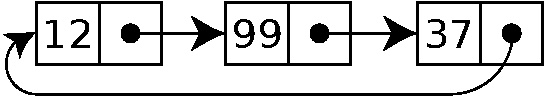
\includegraphics[width=0.45\textwidth]{cyclic-list.pdf}

                  \begin{tiny}
                      \attributionPDWikimedia{https://commons.wikimedia.org/wiki/File:Circularly-linked-list.svg}{Lasindi}
                  \end{tiny}
              \end{center}
    \end{itemize}
\end{frame}

\begin{frame}
    \frametitle{Практика}

    Вместе реализуем односвязный список, оперирующий целыми числами, с~операциями:
    \begin{description}
        \item[insert] Вставить элемент в список по заданному индексу
        \item[get] Получить элемент по заданному индексу
        \item[remove] Удалить элемент по заданному индексу
              % \item[head] Получить первый элемент списка
              % \item[tail] Получить последний элемент списка
        \item[append] Сцепить два списка (если успеем)
    \end{description}
    и служебными функциями:
    \begin{description}
        \item[new] Создать пустой список
        \item[printList] Распечатать содержимое списка
        \item[delete] Удалить весь список (освободить память)
    \end{description}


\end{frame}

\begin{frame}
    \frametitle{Домашнее задание}

    \begin{footnotesize}
        \begin{enumerate}
            \item Написать программу, которая в диалоговом режиме позволяет осуществлять следующие операции:
                  \begin{description}
                      \item[0] выйти
                      \item[1] добавить значение в сортированный список
                      \item[2] удалить значение из списка
                      \item[3] распечатать список
                  \end{description}
                  Все операции должны сохранять сортированность.
                  Начинаем с пустого списка.
            \item Отряд из 41-го сикария, защищавший галилейскую крепость Массада, не пожелал сдаваться в плен блокировавшим его превосходящим силам римлян.
                  Сикарии стали в круг и договорились, что каждые два воина будут убивать третьего, пока не погибнут все.
                  Самоубийство — тяжкий грех, но тот, кто в конце концов останется последним, должен будет его совершить.
                  Иосиф Флавий, командовавший этим отрядом, якобы быстро рассчитал, где нужно стать ему и его другу, чтобы остаться последними, но не для того, чтобы убить друг друга, а чтобы сдать крепость римлянам.
                  В нашем случае участвует n воинов и убивают каждого m-го.
                  Требуется определить номер k начальной позиции воина, который должен будет остаться последним.
                  Считать с помощью циклического списка.
        \end{enumerate}

        Особо обращайте внимание на утечки памяти.
    \end{footnotesize}
\end{frame}

\end{document}
